\documentclass[11pt]{article} 
\usepackage[english]{babel}
\usepackage[utf8]{inputenc}
\usepackage[margin=0.5in,top=0.5in,bottom=0.75in]{geometry}
\usepackage{amsmath}
\usepackage{amsthm}
\usepackage{amsfonts}
\usepackage{amssymb}
\usepackage[usenames,dvipsnames]{xcolor}
\usepackage{graphicx}
\usepackage[siunitx]{circuitikz}
\usepackage{tikz}
\usepackage[colorinlistoftodos, color=orange!50]{todonotes}
\usepackage{hyperref}
\usepackage[numbers, square]{natbib}
\usepackage{fancybox}
\usepackage{epsfig}
\usepackage{soul}
\usepackage[framemethod=tikz]{mdframed}
\usetikzlibrary{positioning, automata, backgrounds}
\usepackage{tikz}\usetikzlibrary{arrows.meta,backgrounds,calc,quotes}
\usepackage[shortlabels]{enumitem}
\usepackage[version=4]{mhchem}
\usepackage{multicol}
\usepackage{forest}
\usepackage{mathtools}
\usepackage{comment}
\usepackage{enumitem}
\usepackage[utf8]{inputenc}
\usepackage[linesnumbered,ruled,vlined]{algorithm2e}
\usepackage{listings}
\usepackage{color}
\usepackage[numbers]{natbib}
\usepackage{subfiles}
\usepackage{tkz-berge}


\newtheorem{prop}{Proposition}[section]
\newtheorem{thm}{Theorem}[section]
\newtheorem{lemma}{Lemma}[section]
\newtheorem{cor}{Corollary}[prop]

\theoremstyle{definition}
\newtheorem{definition}{Definition}

\theoremstyle{definition}
\newtheorem{required}{Problem}
\newtheorem*{requiredHC}{Problem HC}

\theoremstyle{definition}
\newtheorem{ex}{Example}


\setlength{\marginparwidth}{3.4cm}
%#########################################################

%To use symbols for footnotes
\renewcommand*{\thefootnote}{\fnsymbol{footnote}}
%To change footnotes back to numbers uncomment the following line
%\renewcommand*{\thefootnote}{\arabic{footnote}}

% Enable this command to adjust line spacing for inline math equations.
% \everymath{\displaystyle}

% _______ _____ _______ _      ______ 
%|__   __|_   _|__   __| |    |  ____|
%   | |    | |    | |  | |    | |__   
%   | |    | |    | |  | |    |  __|  
%   | |   _| |_   | |  | |____| |____ 
%   |_|  |_____|  |_|  |______|______|
%%%%%%%%%%%%%%%%%%%%%%%%%%%%%%%%%%%%%%%

\title{
\normalfont \normalsize 
\textsc{CSCI 3104 Fall 2022 \\ 
Instructors: Prof. Grochow and Nagesh} \\
[10pt] 
\rule{\linewidth}{0.5pt} \\[6pt] 
\huge Problem Set 3 \\
\rule{\linewidth}{2pt}  \\[10pt]
}
%\author{}
\date{}

\begin{document}

\definecolor{processblue}{cmyk}{0.96,0,0,0}
\definecolor{processred}{rgb}{200, 0, 0}
\definecolor{processgreen}{rgb}{0, 255, 0}
\DeclareGraphicsExtensions{.png}
\DeclareGraphicsExtensions{.gif}
\DeclareGraphicsExtensions{.jpg}

\maketitle


%%%%%%%%%%%%%%%%%%%%%%%%%
%%%%%%%%%%%%%%%%%%%%%%%%%%
%%%%%%%%%%FILL IN YOUR NAME%%%%%%%
%%%%%%%%%%AND STUDENT ID%%%%%%%%
%%%%%%%%%%%%%%%%%%%%%%%%%%
\noindent
Due Date \dotfill September 19, 2022 8pm MT\\
Name \dotfill \textbf{Tyler Huynh} \\
Student ID \dotfill \textbf{109603994} \\
Collaborators \dotfill \textbf{N/A}

\tableofcontents

\section*{Instructions}
\addcontentsline{toc}{section}{Instructions}

 \begin{itemize}
	\item The solutions \textbf{should be typed}, using proper mathematical notation. We cannot accept hand-written solutions. \href{http://ece.uprm.edu/~caceros/latex/introduction.pdf}{Here's a short intro to \LaTeX.}
	\item You should submit your work through the \textbf{class Canvas page} only. Please submit one PDF file, compiled using this \LaTeX \ template.
	\item You may not need a full page for your solutions; pagebreaks are there to help Gradescope automatically find where each problem is. Even if you do not attempt every problem, please submit this document with no fewer pages than the blank template (or Gradescope has issues with it).

	\item You are welcome and encouraged to collaborate with your classmates, as well as consult outside resources. You must \textbf{cite your sources in this document.} \textbf{Copying from any source is an Honor Code violation. Furthermore, all submissions must be in your own words and reflect your understanding of the material.} If there is any confusion about this policy, it is your responsibility to clarify before the due date. 

	\item Posting to \textbf{any} service including, but not limited to Chegg, Reddit, StackExchange, etc., for help on an assignment is a violation of the Honor Code.

	\item You \textbf{must} virtually sign the Honor Code (see Section \ref{HonorCode}). Failure to do so will result in your assignment not being graded.
\end{itemize}


\section*{Honor Code (Make Sure to Virtually Sign)} \label{HonorCode}
\addcontentsline{toc}{section}{Honor Code (Make Sure to Virtually Sign)}
\hypertarget{HonorCode}{}

\begin{requiredHC}
\begin{itemize}
\item My submission is in my own words and reflects my understanding of the material.
\item Any collaborations and external sources have been clearly cited in this document.
\item I have not posted to external services including, but not limited to Chegg, Reddit, StackExchange, etc.
\item I have neither copied nor provided others solutions they can copy.
\end{itemize}

%\noindent In the specified region below, clearly indicate that you have upheld the Honor Code. Then type your name. 
\end{requiredHC}

\begin{proof}[I agree to the above, Tyler Huynh.]
%% Typing "I agree to the above," followed by your name is sufficient.
\end{proof}


\newpage
\setcounter{section}{5}
\section{Standard 6 -- Safe and Useless Edges}

\setcounter{required}{5}
\begin{required}
Consider the weighted graph $G(V, E, w)$ below. Let $\mathcal{F} = \{ \{A, B\}, \{B, G\}, \{E, F\}\}$ be an intermediate spanning forest (indicated by the thick edges below). Label each edge that is \textbf {not} in $\mathcal{F}$ as safe, useless, or undecided. Provide a 1-2 sentence explanation for each such edge.


\begin{center}
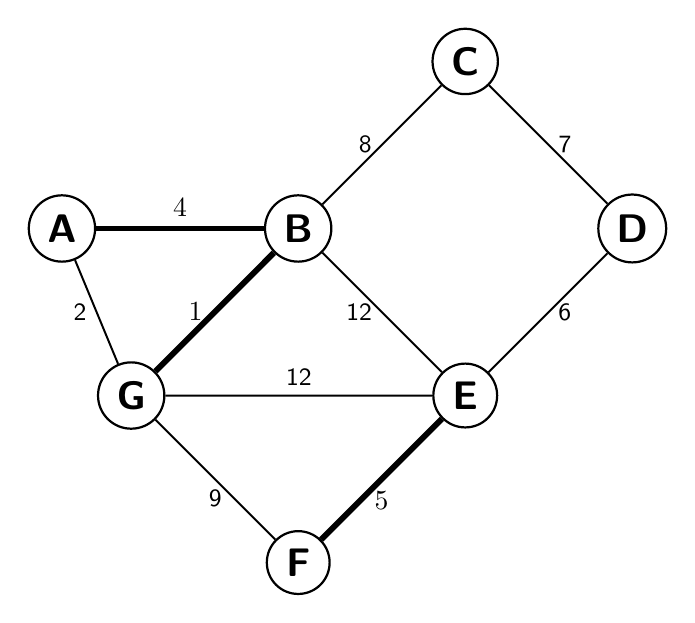
\begin{tikzpicture}[scale=0.4, auto, node distance=3cm, every loop/.style={},
  thick,main node/.style={circle,draw,font=\sffamily\Large\bfseries}]

\node[main node] (A) {A};
\node[main node] (B) [right of=A] {B};
\node[main node] (C) [above right of=B] {C};
\node[main node] (D) [below right of=C] {D};
\node[main node] (E) [below left of=D] {E};
\node[main node] (F) [below left of=E] {F};
\node[main node] (G) [above left of=F] {G};

\path[line width=0.25mm, every node/.style={font=\sffamily\small}]
(B) edge node [left]  {8} (C)
(B) edge node [left]  {12}  (E)
(C) edge node [right] {7}  (D)
(D) edge node [right] {6} (E)
(F) edge node [below] {9} (G)
(G) edge node [above] {12}  (E) 
(A) edge node [left] {2} (G)
;

\draw[line width=0.75mm] (A) -- node [above] {4} (B);
\draw[line width=0.75mm] (E) -- node [below] {5} (F);
\draw[line width=0.75mm] (B) -- node [left] {1} (G);
\end{tikzpicture}
\end{center}
\end{required}

\begin{proof}[Answer] Answer\\
\begin{itemize} 
\item The edge $\{A,G\}$ is... useless \\% safe/useless/undecided
This is because ...this edge from \{A,G\} is useless because by the definition of a useless edge the vertex of A and G both reside in the same spanning forest.
\item The edge $\{G,F\}$ is... safe\\% safe/useless/undecided
This is because ... .this edge is safe because from the vertex {G, F} it would have the minimum edge weight of 9. Further, it is also an edge that is between two different forest . %Your answer here
\item The edge $\{G,E\}$ is... undecided\\% safe/useless/undecided
This is because ... .this edge is safe because from the vertex {G, E} it is not the minimum weight edge, but it is also an edge that is between two different forest .
\item The edge $\{B,E\}$ is... undecided\\% safe/useless/undecided
This is because ... this edge is undecided because it exists in the span of two different forest and  is not a minimum edge weight.%Your answer here
\item The edge $\{B,C\}$ is... safe \\% safe/useless/undecided
This is because ... this edge is safe because there exists a light edge that belongs to the vertex of C, further it is a minimum edge weight as well.%Your answer here
\item The edge $\{C,D\}$ is... undecided \\% safe/useless/undecided
This is because ... This edge would be neither safe or useless since the vertex of c and d do not lie within the spanning forest of \{a, b, g\} or \{e and f\}
\item The edge $\{D,E\}$ is... safe\\% safe/useless/undecided
This is because ... This edge would be safe because there exists a light edge that belongs to the vertex of C, further it is a minimum weight edge weight. %Your answer here
\end{itemize}
\end{proof}


\newpage
\section{Standard 7: Kruskal's MST Algorithm}
\begin{required}
Consider the weighted graph $G(V, E, w)$ below. Clearly list the order in which Kruskal's algorithm adds edges to a minimum-weight spanning tree for $G$. Additionally, clearly articulate the steps that Kruskal's algorithm takes as it selects the first \textbf{three} edges.


\begin{center}
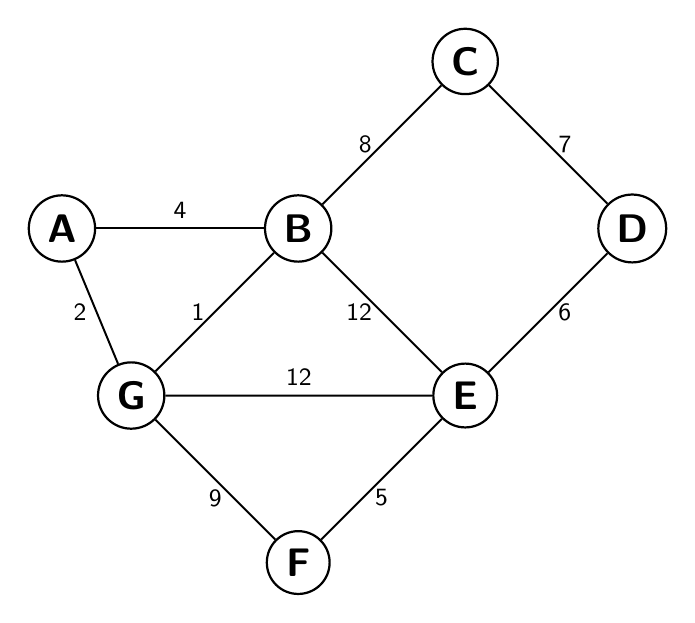
\begin{tikzpicture}[scale=0.4, auto, node distance=3cm, every loop/.style={},
  thick,main node/.style={circle,draw,font=\sffamily\Large\bfseries}]

\node[main node] (A) {A};
\node[main node] (B) [right of=A] {B};
\node[main node] (C) [above right of=B] {C};
\node[main node] (D) [below right of=C] {D};
\node[main node] (E) [below left of=D] {E};
\node[main node] (F) [below left of=E] {F};
\node[main node] (G) [above left of=F] {G};

\path[line width=0.25mm, every node/.style={font=\sffamily\small}]
(B) edge node [left]  {8} (C)
(B) edge node [left]  {12}  (E)
(C) edge node [right] {7}  (D)
(D) edge node [right] {6} (E)
(F) edge node [below] {9} (G)
(G) edge node [left]  {1} (B)
(G) edge node [above] {12}  (E)
(A) edge node [above] {4} (B)
(E) edge node [below] {5} (F)
(A) edge node [left] {2} (G)
;
\end{tikzpicture}
\end{center}
\end{required}

\begin{proof}
Kruskal's algorithm by definition traverses the graph by adding all the vertices with weights to a priority queue organized from least to greatest weights and initialize an empty to a minimum weight spanning tree of G. \\
We will initialize a priority queue containing all the vertices and their respective edge weights:\\
\begin{center}
\begin{tabular}{ | c | c | c | c | c | c | c | c | c | c | c |}
 \hline
 Vertices:& \{G, B\} & \{A, G\} & \{A, B\} & \{E, F\} & \{E, D\} & \{C, D\} & \{B, C\} & \{G, F\} & \{G, E\} & \{B, E\}\\ 
 \hline
 Edge Weights:& 1 & 2 & 4 & 5 & 6 & 7 & 8 & 9 & 12 & 12\\  
 \hline
\end{tabular}
\end{center}

From the above we will now select the edges such that we will create a minimum edge weight spanning tree of G:
\begin{center}
Priority Queue: [\{G, B\}, \{A, G\}, \{A, B\}, \{E, F\}, \{E, D\}, \{C, D\}, \{B, C\}, \{G, F\}, \{G, E\}, \{B, E\}] \\
\end{center}

We will first pop off the vertices of \{G, B\} from our priority queue and check if it creates a cycle, which it does not and add it to our tree of G. \\
\begin{center}
Priority Queue: [\{A, G\}, \{A, B\}, \{E, F\}, \{E, D\}, \{C, D\}, \{B, C\}, \{G, F\}, \{G, E\}, \{B, E\}]\\
Minimum Weight Spanning Tree $G$: [\{G, B\}] \\
\end{center}

We will now pop off the vertices of \{A, G\} from our priority queue and check if it creates a cycle, which it does not and add it to our tree of G. \\
\begin{center}
Priority Queue: [\{A, B\}, \{E, F\}, \{E, D\}, \{C, D\}, \{B, C\}, \{G, F\}, \{G, E\}, \{B, E\}]\\
Minimum Weight Spanning Tree $G$: [\{G, B\}, \{A, G\}] \\
\end{center}

The vertex of \{A, B\} will be popped off the priority queue, but will not be added into the Minimum Weight Spanning Tree of G because it will create a cycle in the graph. . \\
\begin{center}
Priority Queue: [\{E, F\}, \{E, D\}, \{C, D\}, \{B, C\}, \{G, F\}, \{G, E\}, \{B, E\}]\\
Minimum Weight Spanning Tree $G$: [\{G, B\}, \{A, G\}, \{A, B\}] \\
\end{center}

After running the priority queue our Minimum Weight Spanning Tree of G will have this set of vertices within it: \\
\begin{center}
Minimum Weight Spanning Tree $G$: [\{G, B\}, \{A, G\}, \{E, F\}, \{E, D\}, \{C, D\}, \{B, C\}]
\end{center}
The Minimum Weight Spanning Tree of $G$ would look like this:
\begin {center}
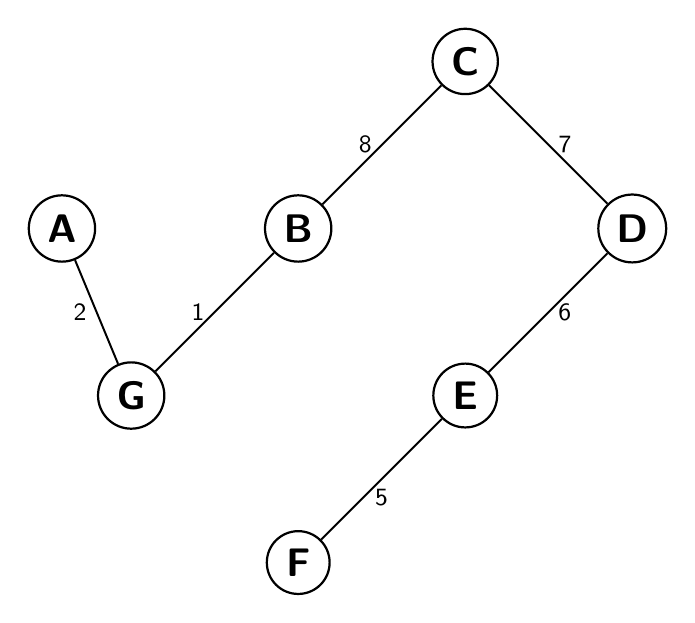
\begin{tikzpicture}[scale=0.4, auto, node distance=3cm, every loop/.style={},
  thick,main node/.style={circle,draw,font=\sffamily\Large\bfseries}]

\node[main node] (A) {A};
\node[main node] (B) [right of=A] {B};
\node[main node] (C) [above right of=B] {C};
\node[main node] (D) [below right of=C] {D};
\node[main node] (E) [below left of=D] {E};
\node[main node] (F) [below left of=E] {F};
\node[main node] (G) [above left of=F] {G};

\path[line width=0.25mm, every node/.style={font=\sffamily\small}]
(B) edge node [left]  {8} (C)
(C) edge node [right] {7}  (D)
(D) edge node [right] {6} (E)
(G) edge node [left]  {1} (B)
(E) edge node [below] {5} (F)
(A) edge node [left] {2} (G)
;
\end{tikzpicture}
\end{center}
\end{proof}


\newpage
\section{Standard 8: Prim's MST Algorithm}
\begin{required}
Consider the weighted graph $G(V, E, w)$ below. Clearly list the order in which Prim's algorithm, \textbf{using the source vertex} $A$, adds edges to a minimum-weight spanning tree for $G$. Additionally, clearly articulate the steps that Prim's algorithm takes as it selects the first \textbf{three} edges.

\begin{center}
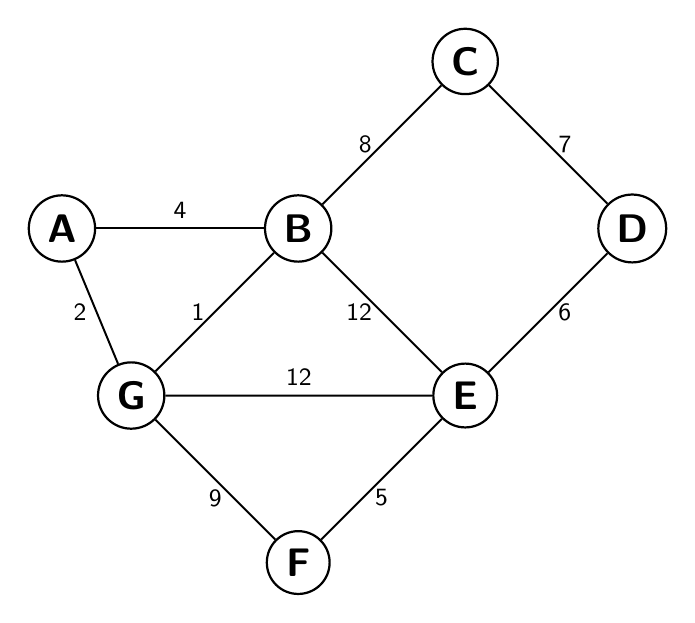
\begin{tikzpicture}[scale=0.4, auto, node distance=3cm, every loop/.style={},
  thick,main node/.style={circle,draw,font=\sffamily\Large\bfseries}]

\node[main node] (A) {A};
\node[main node] (B) [right of=A] {B};
\node[main node] (C) [above right of=B] {C};
\node[main node] (D) [below right of=C] {D};
\node[main node] (E) [below left of=D] {E};
\node[main node] (F) [below left of=E] {F};
\node[main node] (G) [above left of=F] {G};

\path[line width=0.25mm, every node/.style={font=\sffamily\small}]
(B) edge node [left]  {8} (C)
(B) edge node [left]  {12}  (E)
(C) edge node [right] {7}  (D)
(D) edge node [right] {6} (E)
(F) edge node [below] {9} (G)
(G) edge node [left]  {1} (B)
(G) edge node [above] {12}  (E)
(A) edge node [above] {4} (B)
(E) edge node [below] {5} (F)
(A) edge node [left] {2} (G)
;
\end{tikzpicture}
\end{center}
\end{required}

\begin{proof}
Prim's algorithm by definition will traverse the graph by pushing on the source vertex then popping it off and visiting itS neighbors. Then we would check if one endpoint is in our minimum-weight spanning tree and if one is not, then we would add it into our tree, if both are in our minimum-weight spanning tree than it would create a cycle. We would further repeat this process until the priority queue is empty and have achieved our minimum-weight spanning tree. \\


\end{proof}





\newpage
\section{Standard 9: Huffman Coding}
\begin{required}
Consider the following sequence of numbers:
\[
S_n = \begin{cases}
3 & n = 0 \\
6 & n = 1 \\
S_{n-1} + S_{n-2} & n \geq 2.
\end{cases}
\]

For an alphabet $\Sigma = \{a,b,c,d,e,f,g,h\}$ with frequencies given by the first $|\Sigma|$ many numbers $S_0, S_1, \dotsc, S_{|\Sigma|-1}$, give an optimal Huffman code and its corresponding encoding tree. Specify the frequencies of each letter, and for each stage of the algorithm, the subtrees merged at that stage, and the resulting total frequency for the new merged subtree.
\end{required}

\begin{proof}
% YOUR ANSWER HERE
\end{proof}



%%%%%%%%%%%%%%%%%%%%%%%%%%%%%%%%%%%%%%%%%%%%%%%%%%

\end{document} % NOTHING AFTER THIS LINE IS PART OF THE DOCUMENT